\problemText{La Red De Transporte}{Entrada estándar}{Salida estándar}{2 segundos}{}{Kleiber Ttito}{0000FF}

La logística de Amazon para el transporte de paquetes entre sus almacenes es un área sumamente desafiante. Por ello, se ha asignado a Kleiber, un ingeniero timido, la tarea de modelar una red de transporte. Esta red contará con un conjunto de almacenes conectados a través de vias. Además, en esta red debe ser posible transportar paquetes entre cualquier par de almacenes.

En la red modelada, el transporte de paquetes entre dos almacenes a través de una vía puede llevarse a cabo de dos maneras:
 \begin{itemize}
    \item Utilizar los camiones propios de Amazon, que pueden recorrer cualquier distancia durante el transporte. No obstante, el número de estos camiones es limitado.
    \item Utilizar los camiones de contratistas, que están disponibles en cantidad ilimitada. Sin embargo, Amazon debe pagar $1$ sol por cada kilómetro recorrido durante el transporte.
\end{itemize}
Amazon se toma muy en serio su principio de frugalidad, que consiste en hacer más con menos. En este sentido, se busca modelar una red de transporte que minimice el costo máximo de transportar paquetes entre dos almacenes a través de una vía utilizando un camión contratista. ¿Podrías ayudar al tímido Kleiber a modelar esta red de transporte y calcular dicho costo?

\inputText

La primera línea contiene un número entero $t$ $(1 \leq t \leq 100)$, que indica el número de casos de prueba. Cada caso de prueba incluye un número entero $C$ $(1 \leq C \leq 100)$, que representa la cantidad de camiones propios de Amazon, y un número entero $A$ $(C < A \leq 500)$, que representa la cantidad de almacenes en la red de transporte. Finalmente, se proporcionan $A$ líneas, cada una con las coordenadas cartesianas $x_i$ e $y_i$ $(0 \leq x_i, y_i \leq 10000)$, las cuales indican la ubicación de cada almacén en kilómetros.

\outputText

Para cada caso, la salida debe ser una línea que indique el costo máximo de transportar paquetes entre dos almacenes a través de una vía utilizando un camión contratista en la red de transporte modelada. El valor debe presentarse con dos decimales.

\exampleCases

\begin{example}
    \exmp{%%INPUT
        \caseFile{2024/RedDeTransporte/in/1.in}
    }{%%OUTPUT
        \caseFile{2024/RedDeTransporte/out/1.out}
    }%%END-OUTPUT
\end{example}

\explanationText


\textbf{En el primer ejemplo:} El modelo de red de transporte que minimiza el pago máximo a un transportista contratado es el siguiente:

\begin{figure}[h]
    \centering
    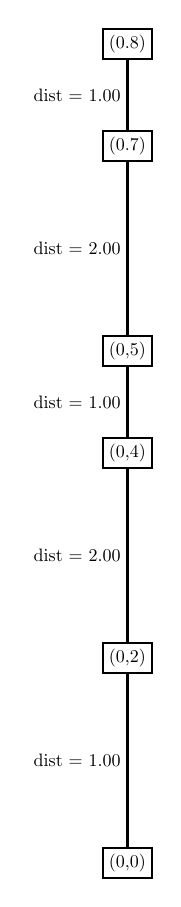
\begin{tikzpicture}[thick,scale=0.65, every node/.style={scale=0.65}]
    \begin{scope}
        \node[draw] (A) at (0,0) {(0,0)};
        \node[draw] (B) at (0,4) {(0,2)};
        \node[draw] (C) at (0,8) {(0,4)};
        \node[draw] (D) at (0,10) {(0,5)};
        \node[draw] (E) at (0,14) {(0.7)};
        \node[draw] (F) at (0,16) {(0.8)};
    \end{scope}

    \begin{scope}
        \draw (A) -- node[midway, left] {dist = 1.00} (B);
        \draw (B) -- node[midway, left] {dist = 2.00} (C);
        \draw (C) -- node[midway, left] {dist = 1.00} (D);
        \draw (D) -- node[midway, left] {dist = 2.00} (E);
        \draw (E) -- node[midway, left] {dist = 1.00} (F);
    \end{scope}
\end{tikzpicture}
\end{figure}

Las distancias de $2.00 km$ son transportadas por los camiones propios de Amazon, mientras que el resto es transportado por contratistas. Por lo tanto, el monto máximo que se pagará a un contratista será de $1.00$ sol.

\textbf{En el segundo ejemplo:} El modelo de red de transporte que minimiza el pago máximo a un transportista contratado es el siguiente:

\begin{figure}[h]
    \centering
    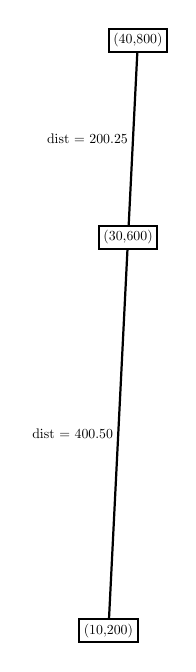
\begin{tikzpicture}[thick,scale=0.5, every node/.style={scale=0.5}]
    \begin{scope}
        \node[draw] (A) at (0.25,5) {(10,200)};
        \node[draw] (B) at (0.75,15) {(30,600)};
        \node[draw] (C) at (1.00,20) {(40,800)};
    \end{scope}

    \begin{scope}
        \draw (A) -- node[midway, left] {dist = 400.50} (B);
        \draw (B) -- node[midway, left] {dist = 200.25} (C);
    \end{scope}
\end{tikzpicture}
\end{figure}

La distancia de $640.31 km$ son transportadas por el camion propio de Amazon, mientras que el resto es transportado por un contratista. Por lo tanto, el monto máximo que se pagará a un contratista será de $492.44$ soles.
